%\documentclass[handout]{beamer}
\documentclass{beamer}\usepackage[]{graphicx}\usepackage[]{color}
%% maxwidth is the original width if it is less than linewidth
%% otherwise use linewidth (to make sure the graphics do not exceed the margin)
\makeatletter
\def\maxwidth{ %
  \ifdim\Gin@nat@width>\linewidth
    \linewidth
  \else
    \Gin@nat@width
  \fi
}
\makeatother

\definecolor{fgcolor}{rgb}{0.345, 0.345, 0.345}
\newcommand{\hlnum}[1]{\textcolor[rgb]{0.686,0.059,0.569}{#1}}%
\newcommand{\hlstr}[1]{\textcolor[rgb]{0.192,0.494,0.8}{#1}}%
\newcommand{\hlcom}[1]{\textcolor[rgb]{0.678,0.584,0.686}{\textit{#1}}}%
\newcommand{\hlopt}[1]{\textcolor[rgb]{0,0,0}{#1}}%
\newcommand{\hlstd}[1]{\textcolor[rgb]{0.345,0.345,0.345}{#1}}%
\newcommand{\hlkwa}[1]{\textcolor[rgb]{0.161,0.373,0.58}{\textbf{#1}}}%
\newcommand{\hlkwb}[1]{\textcolor[rgb]{0.69,0.353,0.396}{#1}}%
\newcommand{\hlkwc}[1]{\textcolor[rgb]{0.333,0.667,0.333}{#1}}%
\newcommand{\hlkwd}[1]{\textcolor[rgb]{0.737,0.353,0.396}{\textbf{#1}}}%
\let\hlipl\hlkwb

\usepackage{framed}
\makeatletter
\newenvironment{kframe}{%
 \def\at@end@of@kframe{}%
 \ifinner\ifhmode%
  \def\at@end@of@kframe{\end{minipage}}%
  \begin{minipage}{\columnwidth}%
 \fi\fi%
 \def\FrameCommand##1{\hskip\@totalleftmargin \hskip-\fboxsep
 \colorbox{shadecolor}{##1}\hskip-\fboxsep
     % There is no \\@totalrightmargin, so:
     \hskip-\linewidth \hskip-\@totalleftmargin \hskip\columnwidth}%
 \MakeFramed {\advance\hsize-\width
   \@totalleftmargin\z@ \linewidth\hsize
   \@setminipage}}%
 {\par\unskip\endMakeFramed%
 \at@end@of@kframe}
\makeatother

\definecolor{shadecolor}{rgb}{.97, .97, .97}
\definecolor{messagecolor}{rgb}{0, 0, 0}
\definecolor{warningcolor}{rgb}{1, 0, 1}
\definecolor{errorcolor}{rgb}{1, 0, 0}
\newenvironment{knitrout}{}{} % an empty environment to be redefined in TeX

\usepackage{alltt}
% ***************************************************************

\usepackage{graphicx}
%\usepackage{psfrag, pstricks}
\usepackage{amsmath,amssymb,array,comment,eucal}
\usepackage{xcolor}
\definecolor{beamer@blendedblue}{RGB}{86,155,189}
\definecolor{myblue}{RGB}{12,76,138}
\setbeamercolor{structure}{fg=myblue}
\definecolor{Ftitle}{RGB}{12,76,138}
\definecolor{Descitem}{RGB}{238,238,244}
\definecolor{StdTitle}{RGB}{12,76,138}
\definecolor{StdBody}{RGB}{213,24,0}
\definecolor{StdBody}{RGB}{213,24,0}

\definecolor{AlTitle}{RGB}{255, 190, 190}
\definecolor{AlBody}{RGB}{213,24,0}

\definecolor{ExTitle}{RGB}{201, 217, 217}
\definecolor{ExBody}{RGB}{213,24,0}

\setbeamercolor{frametitle}{fg = Ftitle}
\setbeamercolor{title}{fg = Ftitle}
\setbeamercolor{item}{fg = Ftitle}
\setbeamercolor{subitem}{fg = Ftitle}
\setbeamercolor{subsubitem}{fg = Ftitle}
\setbeamercolor{description item}{fg = myblue}
\setbeamercolor{titlelike}{fg=myblue}

%$Id: macros.tex,v 1.2 2006/02/13 14:23:55 rlw Exp rlw $
\newcommand{\Lmea}{{\cal L}} 
\newcommand{\scale}{\bflambda} 
\newcommand{\Scale}{\bfLambda} 
\newcommand{\bfscale}{\bflambda} 
\newcommand{\mean}{\bfchi}
\newcommand{\loc}{\bfchi}
\newcommand{\bfmean}{\bfchi}
\renewcommand{\k}{g}
\newcommand{\Gen}{{\cal G}}
\newcommand{\eps}{\epsilon}

\newcommand{\ind}{\mathrel{\mathop{\sim}\limits^{\mathit{ind}}}}
\newcommand{\iid}{\mathrel{\mathop{\sim}\limits^{\mathit{iid}}}}
\newcommand{\dis}{\mathrel{\mathop{=}\limits^{d}}}
\newcommand{\sgn}{\mathop{\rm sgn}}
\newcommand{\cmp}{h}
\newcommand{\dbdo}{d\beta ~ d\omega}
\newcommand{\real}{{\mathbb{R}}}
\newcommand{\Ber}{\mbox{\rm Ber}}
\newcommand{\GP}{\mbox{\rm GP}}
\newcommand{\SaS}{\text{S$\alpha$S}}
\newcommand{\RA}{{\real \times A}}
\newcommand{\RK}{{\real \times K}}
\newcommand{\RO}{{\real \times \Omega}} 
\newcommand{\RS}{{\bbR \times \LamS}}
  \newcommand{\set}[1]{\left\{#1\right\}}
  \newcommand{\bet}[1]{\left[#1\right]}
  \newcommand{\cet}[1]{\left(#1\right)}
%  \renewcommand{\half}{{\scriptstyle\frac12}}
\newcommand{\subA}{(\eps_1 < \beta \le \eps_2) \times \LamS}
 \newcommand{\uu}{{\big(\scale(x - \loc)\big)}}
 \newcommand{\uuj}{{\big(\scale_j(x-\loc_j)\big)}}
 \newcommand{\bbT}{{\mathbb{T}}}
 \newcommand{\ui}{{[0,1)}}
 \newcommand{\spq}[1]{\left|#1\right|^s_{pq}}
 \newcommand{\spqper}[1]{\left|#1\right|^{s\,*}_{pq}}
 \newcommand{\sspqper}[1]{\left\|#1\right\|^{s\,*}_{pq}}
 \newcommand{\sspq}[1]{\left\|#1\right\|^s_{pq}}    % Besov semi-norm
 \newcommand{\qp}[1]  {\left\|#1\right\|^q_p}         % Hilbert-space norm
 \newcommand{\qper}[1]{\left\|#1\right\|^{*\,q}_p}  % Periodic HS norm
 

\newcommand{\bbW}{{\mathbb{W}}}
\newcommand{\bbB}{{\mathbb{B}}}
\newcommand{\Sob}{{\ensuremath{\bbW^s_2}}}
\newcommand{\Besov}{{\ensuremath{\bbB^s_{pq}}}}
\newcommand{\Besper}{{\ensuremath{\bbB^{s\,*}_{pq}}}}
\newcommand{\Sobx}[1]{{\bbW^{#1}_2}}
\newcommand{\Besovx}[1]{{\bbB^{#1}_2}}
\newcommand{\SN}[1]{\|{#1}\|_\Sob}
% MATH LETTER DEFINITIONS
\newcommand{\Levy}{L{\'e}vy}
\newcommand{\nmathbf}{\bm}
\newcommand{\tabb}[1]{\hspace*{#1\parindent}}
%\newcommand{\G}{{g}}    % Really the same as \GB
\newcommand{\g}{{\phi}} %\newcommand{\g}{{g}}
\newcommand{\GB}{{g}}  
% Roman math Bold face 


\def\bfA{\nmathbf A}
\def\bfB{\nmathbf B}
\def\bfC{\nmathbf C}
\def\bfD{\nmathbf D}
\def\bfE{\nmathbf E}
\def\bfF{\nmathbf F}
\def\bfG{\nmathbf G}
\def\bfH{\nmathbf H}
\def\bfI{\nmathbf I}
\def\bfJ{\nmathbf J}
\def\bfK{\nmathbf K}
\def\bfL{\nmathbf L}
\def\bfM{\nmathbf M}
\def\bfN{\nmathbf N}
\def\bfO{\nmathbf O}
\def\bfP{\nmathbf P}
\def\bfQ{\nmathbf Q}
\def\bfR{\nmathbf R}
\def\bfS{\nmathbf S}
\def\bfT{\nmathbf T}
\def\bfU{\nmathbf U}
\def\bfV{\nmathbf V}
\def\bfW{\nmathbf W}
\def\bfX{\nmathbf X}
\def\bfY{\nmathbf Y}
\def\bfZ{\nmathbf Z}

\def\bfa{\nmathbf a}
\def\bfb{\nmathbf b}
\def\bfc{\nmathbf c}
\def\bfd{\nmathbf d}
\def\bfe{\nmathbf e}
\def\bff{\nmathbf f}
\def\bfg{\nmathbf g}
\def\bfh{\nmathbf h}
\def\bfi{\nmathbf i}
\def\bfj{\nmathbf j}
\def\bfk{\nmathbf k}
\def\bfl{\nmathbf l}
\def\bfm{\nmathbf m}
\def\bfn{\nmathbf n}
\def\bfo{\nmathbf o}
\def\bfp{\nmathbf p}
\def\bfq{\nmathbf q}
\def\bfr{\nmathbf r}
\def\bfs{\nmathbf s}
\def\bft{\nmathbf t}
\def\bfu{\nmathbf u}
\def\bfv{\nmathbf v}
\def\bfw{\nmathbf w}
\def\bfx{\nmathbf x}
\def\bfy{\nmathbf y}
\def\bfz{\nmathbf z}


\def\bfalpha  {\nmathbf \alpha}
\def\bfbeta   {\nmathbf \beta}
\def\bfgamma  {\nmathbf \gamma}
\def\bfdelta  {\nmathbf \delta}
\def\bfepsilon{\nmathbf \epsilon}
\def\bfvareps {\nmathbf \varepsilon}
\def\bfzeta   {\nmathbf \zeta}
\def\bfeta    {\nmathbf \eta}
\def\bftheta  {\nmathbf \theta}
\def\bfiota   {\nmathbf \iota}
\def\bfkappa  {\nmathbf \kappa}
\def\bflambda {\nmathbf \lambda}
\def\bfmu     {\nmathbf \mu}
\def\bfnu     {\nmathbf \nu}
\def\bfxi     {\nmathbf \xi}
\def\bfomicron{\nmathbf \omicron}
\def\bfpi     {\nmathbf \pi}
\def\bfrho    {\nmathbf \rho}
\def\bfsigma  {\nmathbf \sigma}
\def\bftau    {\nmathbf \tau}
\def\bfupsilon{\nmathbf \upsilon}
\def\bfphi    {\nmathbf \phi}
\def\bfpsi    {\nmathbf \psi}
\def\bfchi    {\nmathbf \chi}
\def\bfomega  {\nmathbf \omega}
\newcommand{\nubw}{{\tilde\nu}}  % no longer red!
\def\bfAlpha  {\nmathbf \Alpha}
\def\bfBeta   {\nmathbf \Beta}
\def\bfGamma  {\nmathbf \Gamma}
\def\bfDelta  {\nmathbf \Delta}
\def\bfEpsilon{\nmathbf \Epsilon}
\def\bfZeta   {\nmathbf \Zeta}
\def\bfEta    {\nmathbf \Eta}
\def\bfTheta  {\nmathbf \Theta}
\def\bfIota   {\nmathbf \Iota}
\def\bfKappa  {\nmathbf \Kappa}
\def\bfLambda {\nmathbf \Lambda}
\def\bfMu     {\nmathbf \Mu}
\def\bfNu     {\nmathbf \Nu}
\def\bfXi     {\nmathbf \Xi}
\def\bfOmicron{\nmathbf \Omicron}
\def\bfPi     {\nmathbf \Pi}
\def\bfRho    {\nmathbf \Rho}
\def\bfSigma  {\nmathbf \Sigma}
\def\bfTau    {\nmathbf \Tau}
\def\bfUpsilon{\nmathbf \Upsilon}
\def\bfPhi    {\nmathbf \Phi}
\def\bfPsi    {\nmathbf \Psi}
\def\bfChi    {\nmathbf \Chi}
\def\bfOmega  {\nmathbf \Omega}

% Number math Bold face

\newcommand{\bfzero}{{\nmathbf 0}}
\newcommand{\bfone}{{\nmathbf 1}}

% Estimators

\newcommand{\ttheta}{\tilde{\theta}}
\newcommand{\htheta}{\hat{\theta}}
\newcommand{\tbtheta}{\tilde{\bftheta}}
\newcommand{\hbtheta}{\hat{\bftheta}}
\newcommand{\tomega}{\tilde{\omega}}
\newcommand{\homega}{\hat{\omega}}
\newcommand{\tbomega}{\tilde{\bfomega}}
\newcommand{\hbomega}{\hat{\bfomega}}
\newcommand{\tlambda}{\tilde{\lambda}}
\newcommand{\hlambda}{\hat{\lambda}}
\newcommand{\tblambda}{\tilde{\bflambda}}
\newcommand{\hblambda}{\hat{\bflambda}}


% Calligraphic

\newcommand{\mc}[1]{\ensuremath{\mathcal{#1}}}

\newcommand{\cfA}{\mc{A}}
\newcommand{\cfB}{\mc{B}}
\newcommand{\cfC}{\mc{C}}
\newcommand{\cfD}{\mc{D}}
\newcommand{\cfE}{\mc{E}}
\newcommand{\cfF}{\mc{F}}
\newcommand{\cfG}{\mc{G}}
\newcommand{\cfH}{\mc{H}}
\newcommand{\cfI}{\mc{I}}
\newcommand{\cfJ}{\mc{J}}
\newcommand{\cfK}{\mc{K}}
\newcommand{\cfL}{\mc{L}}
\newcommand{\cfM}{\mc{M}}
\newcommand{\cfN}{\mc{N}}
\newcommand{\cfO}{\mc{O}}
\newcommand{\cfP}{\mc{P}}
\newcommand{\cfQ}{\mc{Q}}
\newcommand{\cfR}{\mc{R}}
\newcommand{\cfS}{\mc{S}}
\newcommand{\cfT}{\mc{T}}
\newcommand{\cfU}{\mc{U}}
\newcommand{\cfV}{\mc{V}}
\newcommand{\cfX}{\mc{X}}
\newcommand{\cfY}{\mc{Y}}
\newcommand{\cfZ}{\mc{Z}}

\newcommand{\bmc}[1]{\ensuremath{\boldsymbol{\mathcal{#1}}}}

\newcommand{\bcfA}{\bmc{A}}
\newcommand{\bcfB}{\bmc{B}}
\newcommand{\bcfC}{\bmc{C}}
\newcommand{\bcfD}{\bmc{D}}
\newcommand{\bcfE}{\bmc{E}}
\newcommand{\bcfF}{\bmc{F}}
\newcommand{\bcfG}{\bmc{G}}
\newcommand{\bcfH}{\bmc{H}}
\newcommand{\bcfI}{\bmc{I}}
\newcommand{\bcfJ}{\bmc{J}}
\newcommand{\bcfK}{\bmc{K}}
\newcommand{\bcfL}{\bmc{L}}
\newcommand{\bcfM}{\bmc{M}}
\newcommand{\bcfN}{\bmc{N}}
\newcommand{\bcfO}{\bmc{O}}
\newcommand{\bcfP}{\bmc{P}}
\newcommand{\bcfQ}{\bmc{Q}}
\newcommand{\bcfR}{\bmc{R}}
\newcommand{\bcfS}{\bmc{S}}
\newcommand{\bcfT}{\bmc{T}}
\newcommand{\bcfU}{\bmc{U}}
\newcommand{\bcfV}{\bmc{V}}
\newcommand{\bcfW}{\bmc{W}}
\newcommand{\bcfX}{\bmc{X}}
\newcommand{\bcfY}{\bmc{Y}}
\newcommand{\bcfZ}{\bmc{Z}}

% Special symbols

\newcommand{\reals}{\mbox{\rm I\kern-.20em R}}
\newcommand{\sreals}{\mbox{\small \rm I\kern-.20em R}}
\newcommand{\LamS}{{\cS^d_+}}

% MATHEMATICAL NOTATION

% Operators

\newcommand{\bg}{\;\bigg\vert\;}
\newcommand{\pr}{\mbox{\rm Pr}}
\newcommand{\D}{\mbox{\rm D}}
\newcommand{\E}{\mbox{\rm E}}
\newcommand{\Mo}{\mbox{\rm Mo}}
\newcommand{\Me}{\mbox{\rm Me}}
\newcommand{\Cov}{\mbox{\rm Cov}}
\newcommand{\Var}{\mbox{\rm Var}}
\newcommand{\Corr}{\mbox{\rm Corr}}
\newcommand{\Q}{\mbox{\rm Q}}

% Distributions
\newcommand{\BeBi}{\mbox{\rm BeBi}}
\newcommand{\Be}{\mbox{\rm Be}}
\newcommand{\Bi}{\mbox{\rm Bi}}
\newcommand{\Br}{\mbox{\rm Br}}
\newcommand{\Ca}{\mbox{\rm Ca}}
\newcommand{\Di}{\mbox{\rm Di}}
\newcommand{\Ex}{\mbox{\rm Ex}}
\newcommand{\Fs}{\mbox{\rm Fs}}
\newcommand{\Ga}{\mbox{\sf G}}
\newcommand{\Ge}{\mbox{\rm Ge}}
\newcommand{\GaGa}{\mbox{\rm GaGa}}
\newcommand{\Hy}{\mbox{\rm Hy}}
\newcommand{\IGa}{\mbox{\rm IGa}}
\newcommand{\IPa}{\mbox{\rm IPa}}
\newcommand{\Lo}{\mbox{\rm Lo}}
\newcommand{\Mu}{\mbox{\rm Mu}}
\newcommand{\N}{\mbox{\rm N}}
\newcommand{\NBi}{\mbox{\rm NBi}}
\newcommand{\NGa}{\mbox{\rm NGa}}
\newcommand{\NWi}{\mbox{\rm NWi}}
\newcommand{\Pa}{\mbox{\rm Pa}}
\newcommand{\Po}{\mbox{\sf P}}
\newcommand{\PoGa}{\mbox{\rm PoGa}}
\newcommand{\Ra}{\mbox{\rm Ra}}
\newcommand{\REx}{\mbox{\rm REx}}
\newcommand{\St}{\mbox{\rm St}}
\newcommand{\Un}{\mbox{\rm Un}}
\newcommand{\Wi}{\mbox{\rm Wi}}

% General Mathematics

\newcommand{\dd}[1]{\,d{#1}}
\newcommand{\barx}{\ensuremath{\bar{x}}}
\newcommand{\comb}[2]{{#1\choose#2}}
\newcommand{\ontop}[2]{{#1\atop#2}}
\newcommand{\h}{{\small\ensuremath{1\over2}}}
\newcommand{\hh}[2]{{\small\ensuremath{#1\over#2}}}

\newcommand{\fn}[1]{\hbox{\textrm{#1}}}
\newcommand{\cred}{\fn{Cr}}
\newcommand\dlim{\mathop{\rm \hbox{$\delta$}lim}}
\newcommand{\goto}{\rightarrow}
\newcommand{\gotoinf}{\rightarrow \infty}

\newcommand{\data}{\ensuremath{\bfx=\{x_1,\ldots,x_n\}}}
\newcommand{\brow}[2]{\ensuremath{\{{#1}_1,\ldots,{#1}_{#2}\}}}
\newcommand{\prow}[2]{\ensuremath{({#1}_1,\ldots,{#1}_{#2})}}

\newcommand{\met}{\thinspace{\rm m}}\newcommand{\km}{\thinspace{\rm km}}
\newcommand{\xbar}{\overline X}%
\newcommand{\xbbar}{\overline{\overline X}}%
\font\ss=cmss12
 \newcommand{\OFP}{(\Omega,\cF,\P)}
 \newcommand{\bbC}{\mathbb{C}}
 \newcommand{\bbF}{\mathbb{F}}
 \newcommand{\bbN}{\mathbb{N}}
 \newcommand{\bbR}{\mathbb{R}}
 \newcommand{\bbX}{\mathbb{X}}
 \newcommand{\bbZ}{\mathbb{Z}}
 \newcommand{\one}[1]{\mathbf{1}_{\{#1\}}}
 \newcommand{\cA}{{\cal A}}
 \newcommand{\cB}{{\cal B}} 
 \newcommand{\cE}{{\cal E}}
 \newcommand{\cF}{{\cal F}}
 \newcommand{\cG}{{\cal G}}
 \newcommand{\cH}{{\cal H}}
 \newcommand{\cM}{{\cal M}}
 \newcommand{\cR}{{\cal R}}
 \newcommand{\cS}{{\cal S}}
 \newcommand{\cT}{{\cal T}}
 \newcommand{\cX}{{\cal X}}
 \newcommand{\cY}{{\cal Y}}
 \newcommand{\cZ}{{\cal Z}}
 \newcommand{\eF}{{\CMcal F}}
 \newcommand{\eG}{{\CMcal G}} 
 \newcommand{\eH}{{\CMcal H}}
 \renewcommand{\P}{{\sf{P}}} 
 \renewcommand{\E}{{\sf{E}}}
 \newcommand{\Ev}{{\sf{Ev}}}%
 \newcommand{\V}{{\sf{V}}} 
 \renewcommand{\Cov}{{\sf{Cov}}}
 %\newcommand{\Be}{\textsf{Be}}
 %\newcommand{\Bi}{\textsf{Bi}}
 %\newcommand{\Ex}{\textsf{Ex}}\newcommand{\Ga}{\textsf{Ga}}
 %\newcommand{\Di}{\textsf{Di}}\newcommand{\Ge}{\textsf{Ge}}
 %\newcommand{\IG}{\textsf{IG}}\newcommand{\Lv}{\textsf{Lv}}
 %\newcommand{\HG}{\textsf{HG}}\newcommand{\MN}{\textsf{MN}}
\newcommand{\NB}{\textsf{NB}}\newcommand{\No}{\textsf{N}}
\newcommand{\LN}{\textsf{LN}}
\newcommand{\Lv}{\mbox{\rm Lv}}
%\newcommand{\Pa}{\textsf{Pa}}
% \newcommand{\Po}{\textsf{Po}}\newcommand{\Un}{\textsf{Un}}
 \newcommand{\argmax}{\textrm{argmax}}
 \renewcommand{\th}{{\ensuremath^{\mbox{\tiny th}}}}
 \newcommand{\nd}{{\ensuremath^{\mbox{\tiny nd}}}}
 \newcommand{\st}{{\ensuremath^{\mbox{\tiny st}}}}
 \newcommand{\ii}{{\ensuremath{\bar{i}}}}% \newcommand{\ii}{{\hat i}}
 \newcommand{\jj}{{\ensuremath{\bar{j}}}}%
 \newcommand{\R}{\texttt{R}}
 \newcommand{\mayeq}{\mathrel{\mathop{=}\limits^?}}
 \newcommand{\pperp}{\mathrel{{\rlap{$~\perp$}\perp\,\,}}}
 \newbox\asbox
 \setbox\asbox=\hbox{\vrule height 15pt depth3.5pt width0pt}
 \def\astrut{\relax\ifmmode\copy\strutbox\else\unhcopy\strutbox\fi}
 \def\Strut{\vrule width0pt height 16pt depth 4pt}%
%\font\tinyss=cmss8 at 8truept % for ^T etc
\newcommand{\tsf}[1]{\textsf{\tiny{#1}}}
\newcommand{\fxa}{\mbox{$f(x\mid\alpha)$}}
\newcommand{\fxt}{\mbox{$f(x\mid\theta)$}}
\newcommand{\fxat}{\mbox{$f(x\mid\alpha,\theta)$}}
\newcommand{\tp}{^{\tsf{T}}}
\newcommand{\as}{\textit{a.s.}}
\newcommand{\ie}{\textit{i.e.{}}}
\newcommand{\etc}{\textit{etc}}
\newcommand{\eg}{\textit{e.g.{}}}%
\newcommand{\half}{{\frac12}}
\newcommand{\Sec}[1]{Section\thinspace(\ref{#1})}
\newcommand{\Thm}[1]{Theorem\thinspace\ref{#1}}
\newcommand{\Cor}[1]{Corollary\thinspace\ref{#1}}
\newcommand{\Eqn}[1]{Equation\thinspace(\ref{#1})}
\newcommand{\Fig}[1]{Figure\thinspace(\ref{#1})}
\newcommand{\Figs}[2]{Figures\thinspace(\ref{#1}) and (\ref{#2})}
\newcommand{\Figab}[2]{Figure\thinspace(\ref{#1}#2)}
\newcommand{\Tab}[1]{Table\thinspace(\ref{#1})}
\newcommand{\jth}{{\ensuremath j^{\mbox{\tiny th}}}}%
\providecommand{\ij}{_{ij}} \newcommand{\ji}[1]{_{ij#1}}%
\newcount\ola \newcount\olb \newcount\olc \newcount\old \newcount\ole
\newcount\och\newcount\level
\newtheorem{cor}{Corollary}
\newtheorem{define}{Definition}
\newtheorem{lem}{Lemma}
\newtheorem{prob}{Problem}
\newtheorem{prop}{Proposition}
\newtheorem{thm}{Theorem}
\def\OL#1{\par\noindent\hangindent=#1\parindent % Outline
  \kern1\hangindent\ignorespaces}%
\def\ol#1{%
    \level=#1
    \ifcase\level
    \ola=0 \olb=0 \olc=0 \old=0 \ole=0\or         % Level 0 (reset)
    \olb=0 \olc=0 \old=0 \ole=0 \advance\ola by 1 % Level 1
    \gdef\olev{\uppercase\expandafter{\romannumeral\ola}} \or
    \olc=0 \old=0 \ole=0 \advance\olb by 1        % Level 2
    \och=64 \advance\och by\olb
    \gdef\olev{\char\och}\or
    \old=0 \ole=0 \advance\olc by 1               % Level 3
    \och=48 \advance\och by\olc
    \gdef\olev{\char\och}\or
    \ole=0 \advance\old by 1                      % Level 4
    \och=96 \advance\och by\old
    \gdef\olev{\char\och}\or
    \advance\ole by 1                             % Level 5
    \gdef\olev{\romannumeral\ole} \or
    \message{Outline depth too deep: #1}\fi
    \ifnum\level>0 \OL\level\llap{\olev.\enspace}\ignorespaces\fi}%
\long\def\comment#1/*#2*/{\endcomment}%
\def\endcomment{\relax}%
%
\makeatletter % Find hours (count1) and minutes (count2) past midnight:
\count1\time \divide\count1 60 \count2=-\count1
\multiply\count2 60 \advance\count2 \time
\edef\now{\two@digits{\the\count1}:\two@digits{\the\count2}}
%\renewcommand\section{\@startsection     % Smaller and sans-serif
%    {section}{1}{\z@}{-3.5ex \@plus -1ex \@minus -.2ex}%
%    {2.3ex \@plus.2ex}{\normalfont\large\bfseries\sffamily}}
%\renewcommand\subsection{\@startsection
%    {subsection}{2}{\z@}{-3.25ex\@plus -1ex \@minus -.2ex}%
%    {1.5ex \@plus .2ex}{\normalfont\large\bfseries\sffamily}}
%\renewcommand\subsubsection{\@startsection
%    {subsubsection}{3}{\z@}{-3.25ex\@plus -1ex \@minus -.2ex}%
%    {1.5ex \@plus .2ex}{\normalfont\normalsize\bfseries\sffamily}}
%\def\@seccntformat#1{\csname the#1\endcsname.\quad} % Add . to sec num's
%\long\def\@makecaption#1#2{%                          Use . not : in cap'ns
%  \vskip\abovecaptionskip
%  \sbox\@tempboxa{#1. #2}%
%  \ifdim \wd\@tempboxa >\hsize
%    #1. #2\par
%  \else
%    \global \@minipagefalse
%    \hb@xt@\hsize{\hfil\box\@tempboxa\hfil}%
%  \fi
%  \vskip\belowcaptionskip}
% BEAMER FIX START
\def\newblock{\beamer@newblock}
% BEAMER FIX END
\makeatother

\def\wbox#1#2#3{{\vcenter{\vbox{\hrule height.#3pt
    \hbox{\vrule width.#3pt height#1pt \kern#2pt \vrule width.#3pt}%
                            \hrule height.#3pt}}}}%
\def\Proof.{\medbreak\noindent{\bf Proof.\enspace}}
\def\qed{{\nobreak\hfill\penalty0\hbox to1truecm{}\nobreak
    \hfill$\wbox634$\par\bigskip}}%

\title{Bayesian Variable Selection}

\author{Hoff Chapter 9,  Mixtures of g-Priors Liang et al JASA}
\date{\today}
%\Logo(-1.9,7.3){
\includegraphics[width=.5in]{../eps/duke}}
% Optional: text to put in the bottom of each slide.
% By default, the title of the talk will be placed there.
%\slideCaption{\textit{October 28, 2005 }}
\IfFileExists{upquote.sty}{\usepackage{upquote}}{}
\begin{document}
% make the title slide
\maketitle
\begin{frame}[fragile]  \frametitle{US Air Example}

\begin{knitrout}
\definecolor{shadecolor}{rgb}{0.969, 0.969, 0.969}\color{fgcolor}

{\centering 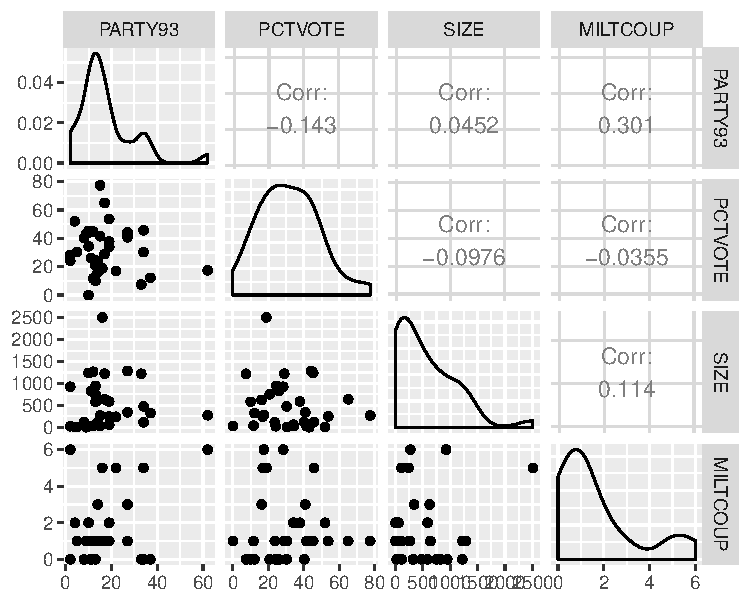
\includegraphics[width=\maxwidth]{figure/data-1} 

}



\end{knitrout}

\end{frame}

\begin{frame}[fragile] \frametitle{lm summary}
\begin{knitrout}
\definecolor{shadecolor}{rgb}{0.969, 0.969, 0.969}\color{fgcolor}\begin{kframe}
\begin{verbatim}
lm(formula = log(SO2) ~ temp + log(firms) + log(popn) + wind +  
    precip + rain, data = usair) 
Coefficients: 
              Estimate Std. Error t value Pr(>|t|)     
(Intercept)  6.7142760  1.6475086   4.075 0.000261 *** 
temp        -0.0649495  0.0227711  -2.852 0.007333 **  
log(firms)   0.3698588  0.1934076   1.912 0.064289 .   
log(popn)   -0.1771293  0.2335520  -0.758 0.453428     
wind        -0.1738606  0.0656713  -2.647 0.012204 *   
precip       0.0156032  0.0132718   1.176 0.247893     
rain         0.0009153  0.0057335   0.160 0.874104     
--- 
Signif. codes:  0 '***' 0.001 '**' 0.01 '*' 0.05 '.' 0.1 ' ' 1 
 
Residual standard error: 0.5108 on 34 degrees of freedom 
Multiple R-squared:  0.5503,	Adjusted R-squared:  0.471  
F-statistic: 6.936 on 6 and 34 DF,  p-value: 7.12e-05 
 
\end{verbatim}
\end{kframe}
\end{knitrout}

\end{frame}

\begin{frame}\frametitle{Zellner's g-prior}
  Centered model:  $$\Y = \1 \alpha + \X^c \b + \epsilon$$
  where $\X^c$ is the centered design matrix where all variables have
  had their mean subtracted \pause
\begin{itemize}
\item  $p(\phi) \propto 1/\phi$  \pause
\item   $p(\alpha \mid \phi) \propto 1$ \pause
\item  $\b \mid \alpha, \phi, \g \sim \N(0, g \phi^{-1}
  ({\X^c}^\prime \X^c)^{-1})$ \pause
%\item  take $g=n$
\end{itemize}

$$\b \mid \Y, \alpha, \phi \sim N\left(\frac{g}{1 + g} \bhat, \phi^{-1}\frac{g}{1 + g} (\X^T\X)^{-1} \right)$$
$$ \phi \mid \Y \sim \Gam \left(\frac{n-1}{2}, \frac{\SSE - \frac{1}{1 + g} \bhat^T (\X^T\X) \bhat}{2} \right) $$
\end{frame}

\begin{frame} \frametitle{joint posterior draws of beta's}
\begin{knitrout}
\definecolor{shadecolor}{rgb}{0.969, 0.969, 0.969}\color{fgcolor}

{\centering \includegraphics[width=\maxwidth]{figure/sim-1} 

}



\end{knitrout}

\end{frame}


\begin{frame} \frametitle{Bayesian Variable Selection}
  \begin{itemize}
   \item Avoid the use of redundant variables (problems with
    interpretations) \pause
   \item Inclusion of un-necessary terms yields less precise
  estimates, particularly if explanatory variables are highly
  correlated with each other \pause
  \item reduced MSE: reduced variance but possibly higher bias  \pause
  \item it is too ``expensive'' to use all variables
  \end{itemize}
\end{frame}


\begin{frame}\frametitle{Bayesian Model Choice}
  \begin{itemize}
  \item
Models for the variable selection problem  are based on a subset of
  the $\X_1, \ldots \X_p$ variables  \pause

\item Encode models with a  vector $\g = (\gamma_1, \ldots
  \gamma_p)$  where  $\gamma_j \in \{0,1\}$
  is an indicator for whether variable $\X_j$ should be included in
  the model $\Mg$.  $\gamma_j = 0 \Leftrightarrow \beta_j
  = 0$  \pause
\item Each value of $\g$ represents one of the $2^p$ models.
\pause
\item Under model $\Mg$:
 $$\Y \mid \alpha, \b, \sigma^2, \g \sim \N(\one \alpha + \Xg \b_\gamma,
 \sigma^2 \I) $$
Where $\Xg$ is design matrix  using the columns in $\X$ where
 $\gamma_j = 1$ and $\b_{\g}$ is the subset of $\b$ that are non-zero.

\end{itemize}

\end{frame}


\begin{frame}\frametitle{Posterior Probabilities of Models}

  \begin{itemize}
  \item Posterior model probabilities
$$p(\M_j \mid \Y) = \frac{ p(\Y \mid \M_j)p(\M_j)}{\sum_jp(\Y \mid
  \M_j)p(\M_j)} $$ \pause
Marginal likelihod of a model is proportional to
$$ p(\Y \mid \Mg) = \iint p(\Y \mid \b_\gamma,
  \sigma^2)p(\b_\gamma \mid \g, \sigma^2)p(\sigma^2 \mid \g)
  d\b\, d\sigma^2$$\pause
  \item Probability $\beta_j \ne 0$: $\sum_{\M_j:  \beta_j \ne 0}
    p(\M_j \mid \Y)$ (marginal posterior inclusion probability) \pause
  \end{itemize}
\end{frame}


\begin{frame}\frametitle{Prior Distributions}
  \begin{itemize}
  \item Bayesian Model choice requires  proper prior distributions on
  regression coefficients (exception parameters that are included in all models) \pause
  \item Vague but proper priors may lead to paradoxes! \pause
  \item Conjugate Normal-Gammas lead to closed form expressions for
  marginal likelihoods, Zellner's g-prior is one of the most popular.
  \end{itemize}

\end{frame}
\begin{frame}\frametitle{Zellner's g-prior within Models}
Centered model:  $$\Y = \1 \alpha + \Xg^c \b_\gamma + \epsilon$$

\begin{itemize}
\item Common parameters $$p(\alpha, \phi) \propto \phi^{-1}$$  \pause
\item Model Specific parameters
$$\b_\gamma \mid \alpha, \phi, \g \sim \N(0, g \phi^{-1}
  ({\Xg^c}^\prime \Xg^c)^{-1})$$ \pause
%\item  take $g=n$
\item Marginal likelihood of $\Mg$  is proportional
to $$ p(\Y \mid \Mg) = C (1 + g)^{\frac{n-p-1}{2}} ( 1 + g (1 -
 R^2_\gamma))^{- \frac{(n-1)}{2}}$$
where $R^2_\gamma$ is the usual $R^2$ for model $\Mg$ and $C$ is a constant that is $p(\Y \mid \M_0)$ (model with intercept alone)
\pause
\item  uniform distribution over space of models $p(\Mg) = 1/(2^p)$
\end{itemize}
\end{frame}

\begin{frame}[fragile] \frametitle{USair Data: Enumeration of All Models}
\begin{knitrout}
\definecolor{shadecolor}{rgb}{0.969, 0.969, 0.969}\color{fgcolor}\begin{kframe}
\begin{alltt}
\hlkwd{library}\hlstd{(devtools)}
\hlkwd{suppressMessages}\hlstd{(}\hlkwd{install_github}\hlstd{(}\hlstr{"merliseclyde/BAS"}\hlstd{))}  \hlcom{# current version}
\hlkwd{library}\hlstd{(BAS)}
\hlstd{poll.bma} \hlkwb{=} \hlkwd{bas.lm}\hlstd{(}\hlkwd{log}\hlstd{(SO2)} \hlopt{~} \hlstd{temp} \hlopt{+} \hlkwd{log}\hlstd{(firms)} \hlopt{+}
                             \hlkwd{log}\hlstd{(popn)} \hlopt{+} \hlstd{wind} \hlopt{+}
                             \hlstd{precip}\hlopt{+} \hlstd{rain,}
                  \hlkwc{data}\hlstd{=usair,}
                  \hlkwc{prior}\hlstd{=}\hlstr{"g-prior"}\hlstd{,}
                  \hlkwc{alpha}\hlstd{=}\hlnum{41}\hlstd{,}    \hlcom{# g = n}
                  \hlkwc{n.models}\hlstd{=}\hlnum{2}\hlopt{^}\hlnum{7}\hlstd{,}\hlcom{# enumerate (can omit)}
                  \hlkwc{method}\hlstd{=}\hlstr{"deterministic"}\hlstd{)}   \hlcom{# fast enumeration}
\end{alltt}
\end{kframe}
\end{knitrout}

\end{frame}

\begin{frame}\frametitle{residual plot)}
\begin{knitrout}
\definecolor{shadecolor}{rgb}{0.969, 0.969, 0.969}\color{fgcolor}\begin{kframe}
\begin{alltt}
\hlkwd{plot}\hlstd{(poll.bma,} \hlkwc{which}\hlstd{=}\hlnum{1}\hlstd{)}
\end{alltt}
\end{kframe}

{\centering \includegraphics[width=\maxwidth]{figure/resplots-1} 

}



\end{knitrout}
\end{frame}

\begin{frame}\frametitle{Model Complexity)}
\begin{knitrout}
\definecolor{shadecolor}{rgb}{0.969, 0.969, 0.969}\color{fgcolor}\begin{kframe}
\begin{alltt}
\hlkwd{plot}\hlstd{(poll.bma,} \hlkwc{which}\hlstd{=}\hlnum{3}\hlstd{)}
\end{alltt}
\end{kframe}

{\centering \includegraphics[width=\maxwidth]{figure/sizeplots-1} 

}



\end{knitrout}
\end{frame}

\begin{frame}\frametitle{Inclusion Probabilities)}
\begin{knitrout}
\definecolor{shadecolor}{rgb}{0.969, 0.969, 0.969}\color{fgcolor}\begin{kframe}
\begin{alltt}
\hlkwd{plot}\hlstd{(poll.bma,} \hlkwc{which}\hlstd{=}\hlnum{4}\hlstd{)}
\end{alltt}
\end{kframe}

{\centering \includegraphics[width=\maxwidth]{figure/pipplots-1} 

}



\end{knitrout}
\end{frame}


\begin{frame}[fragile]\frametitle{Model Space}
\begin{knitrout}
\definecolor{shadecolor}{rgb}{0.969, 0.969, 0.969}\color{fgcolor}\begin{kframe}
\begin{alltt}
\hlkwd{summary}\hlstd{(poll.bma)}
\end{alltt}
\begin{verbatim}
##            P(B != 0 | Y)  model 1   model 2    model 3   model 4   model 5
## Intercept      1.0000000 1.000000 1.0000000 1.00000000 1.0000000 1.0000000
## temp           0.9762282 1.000000 1.0000000 1.00000000 1.0000000 1.0000000
## log(firms)     0.7659857 1.000000 1.0000000 1.00000000 1.0000000 1.0000000
## log(popn)      0.4075393 0.000000 1.0000000 1.00000000 0.0000000 0.0000000
## wind           0.8080832 1.000000 1.0000000 1.00000000 1.0000000 1.0000000
## precip         0.6615960 1.000000 1.0000000 1.00000000 1.0000000 0.0000000
## rain           0.4166394 0.000000 0.0000000 1.00000000 1.0000000 1.0000000
## BF                    NA 1.000000 0.2093987 0.03277353 0.1544798 0.3022674
## PostProbs             NA 0.209600 0.1097000 0.10300000 0.0809000 0.0634000
## R2                    NA 0.542700 0.5500000 0.55030000 0.5427000 0.5130000
## dim                   NA 5.000000 6.0000000 7.00000000 6.0000000 5.0000000
## logmarg               NA 7.616228 6.0527128 4.19809382 5.7485360 6.4197847
\end{verbatim}
\end{kframe}
\end{knitrout}
\end{frame}


\begin{frame}\frametitle{Summary}
\begin{knitrout}
\definecolor{shadecolor}{rgb}{0.969, 0.969, 0.969}\color{fgcolor}\begin{kframe}
\begin{alltt}
\hlkwd{image}\hlstd{(poll.bma)}
\end{alltt}
\end{kframe}

{\centering \includegraphics[width=\maxwidth]{figure/summary-1} 

}



\end{knitrout}
\end{frame}

\begin{frame}[fragile] \frametitle{Coefficients}
\begin{knitrout}
\definecolor{shadecolor}{rgb}{0.969, 0.969, 0.969}\color{fgcolor}\begin{kframe}
\begin{alltt}
 \hlstd{beta} \hlkwb{=} \hlkwd{coef}\hlstd{(poll.bma,} \hlkwc{n.models}\hlstd{=}\hlnum{1}\hlstd{)}
 \hlstd{beta}
\end{alltt}
\begin{verbatim}
## 
##  Marginal Posterior Summaries of Coefficients: 
## 
##  Based on the top  1 models 
##             post mean  post SD   post p(B != 0)
## Intercept    3.15300    0.07818   1.00000      
## temp        -0.07130    0.01268   0.97623      
## log(firms)   0.23428    0.08573   0.76599      
## log(popn)    0.00000    0.00000   0.40754      
## wind        -0.17998    0.06128   0.80808      
## precip       0.01884    0.00729   0.66160      
## rain         0.00000    0.00000   0.41664
\end{verbatim}
\end{kframe}
\end{knitrout}
\end{frame}

\begin{frame}[fragile] \frametitle{Coefficients}
\begin{knitrout}
\definecolor{shadecolor}{rgb}{0.969, 0.969, 0.969}\color{fgcolor}\begin{kframe}
\begin{alltt}
 \hlkwd{par}\hlstd{(}\hlkwc{mfrow}\hlstd{=}\hlkwd{c}\hlstd{(}\hlnum{2}\hlstd{,}\hlnum{2}\hlstd{));}  \hlkwd{plot}\hlstd{(beta,} \hlkwc{subset}\hlstd{=}\hlkwd{c}\hlstd{(}\hlnum{3}\hlstd{,} \hlnum{6}\hlstd{))}
\end{alltt}
\end{kframe}
\includegraphics[width=\maxwidth]{figure/coefplot-1} 

\end{knitrout}

\end{frame}

\begin{frame}[fragile] \frametitle{Bayesian Confidence Intervals}
\begin{knitrout}
\definecolor{shadecolor}{rgb}{0.969, 0.969, 0.969}\color{fgcolor}\begin{kframe}
\begin{alltt}
\hlkwd{confint}\hlstd{(beta)}
\end{alltt}
\begin{verbatim}
##                  2.5  %     97.5  %        beta
## Intercept   2.994993257  3.31101398  3.15300362
## temp       -0.096926645 -0.04567203 -0.07129934
## log(firms)  0.061014518  0.40753936  0.23427694
## log(popn)   0.000000000  0.00000000  0.00000000
## wind       -0.303835463 -0.05612195 -0.17997871
## precip      0.004105874  0.03357242  0.01883915
## rain        0.000000000  0.00000000  0.00000000
## attr(,"Probability")
## [1] 0.95
## attr(,"class")
## [1] "confint.bas"
\end{verbatim}
\end{kframe}
\end{knitrout}
\end{frame}

\end{document}


\begin{frame}
  \frametitle{Problem with g Prior}



The Bayes factor for comparing $\Mg$ to the null
model:
$$
 BF(\Mg : \M_0) =    (1 + g)^{(n - 1 - p_\g)/2} (1 + g(1 - \R^2))^{(n-1)/2}
$$

\begin{itemize}
\item Let $g$ be a fixed constant and take $n$ fixed.
\item Let $F = \frac{R_g^2/\pg}{(1 - R_\g^2)/(n - 1 - \pg)}$
\item As $R^2_\g \to 1$, $F \to \infty$ LR test would reject $H_0$
\end{itemize}


usual $F$ statistic for  comparing model $\Mg$ to $\M_0$

\end{frame}
\section{Mortality}
\begin{frame}[fragile]
\frametitle{Mortality \& Pollution}
  \begin{itemize}
  \item Data from Statistical Sleuth 12.17 \pause
  \item 60 cities \pause
\item response Mortality \pause
\item measures of HC, NOX, SO2 \pause
\item Is pollution associated with mortality after adjusting for other
  socio-economic and meteorological factors? \pause
\item 15 predictor variables implies $2^{15} = 32,768$ possible models
  \pause
\item Use Zellner-Siow Cauchy prior  $1/g \sim  G(1/2, n/2)$
  \end{itemize}
\begin{verbatim}
mort.bma = bas.lm(MORTALITY ~ ., data=mortality,
                  prior="ZS-null",
                  alpha=60,  n.models=2^15,
                  update=100, initprobs="eplogp")
\end{verbatim}
\end{frame}

\begin{frame}\frametitle{Posterior Distributions}
  \includegraphics[height=3.5in]{mort-sum}
\end{frame}



\begin{frame}[fragile]
\frametitle{Posterior Probabilities}
  \begin{itemize}
  \item What is the probability that there is no pollution effect? \pause
\item Sum posterior model probabilities over all models that include
  no pollution variables \pause
\begin{verbatim}
> which.mat = list2matrix.which(mort.bma,1:(2^15))
> poll.in = (which.mat[, 14:16] %*% rep(1, 3)) == 0
> sum(poll.in * mort.bma$postprob)
[1] 0.9889641
\end{verbatim}\pause
\item Posterior probability is $0.011$ \pause
\item Odds that there is an effect  $(1 - .011)/(.011) = 89.6$ \pause
\item Prior Odds $7.9 = (1 - .2^3)/.2^3$ \pause
\item Bayes Factor for a pollution effect $ 89.6/7.9 = 11.3$ \pause
\item Bayes Factor for NOX based on marginal inclusion probability
  $0.917/(1 - 0.917) = 11.0$ \pause
\item Marginal inclusion probability for logHC =  0.427144
\item Marginal inclusion probability for logSO2 = 0.218978
\end{itemize}
Bayes Factors are not additive!
\end{frame}
\begin{frame}\frametitle{Model Space}
  \includegraphics[height=3.5in]{mort-image}
\end{frame}
\begin{frame}\frametitle{Coefficients}
  \includegraphics[height=3.5in]{mort-beta1}
\end{frame}

\begin{frame}\frametitle{Coefficients}
  \includegraphics[height=3.5in]{mort-beta2}
\end{frame}

\begin{frame}
  \frametitle{Effect Estimation}
  \begin{itemize}
  \item  Coefficients in each model are adjusted for other variables
    in the model
\item OLS:  leave out a predictor with a non-zero coefficient then
  estimates are biased!
\item Model Selection in the presence of high correlation, may leave
  out "redundant" variables;
\item improved MSE for prediction (Bias-variance tradeoff)
\item Bayes is biased anyway so should we care?
\item What is meaning of $\sum_{\g} \beta_{j \g} \gamma_j P(\Mg \mid \Y)$
  \end{itemize}
  Problem with confounding!  Need to change prior?

\end{frame}

\begin{frame}\frametitle{Model Selection}
  Selection of a single model has the following problems \pause
  \begin{itemize}
  \item When the criteria suggest that several models are equally
    good, what should we report?  Still pick only one model? \pause
\item What do we report for our uncertainty after selecting a model?  \pause
  \end{itemize}
Typical analysis ignores model uncertainty! \pause
\vfill

Winner's Curse
\end{frame}


\begin{frame}\frametitle{ Other Problems}


  \begin{itemize}
  \item Computational \pause
  if $p > 35$  enumeration is difficult \pause
  \begin{itemize}
  \item Gibbs sampler or Random-Walk algorithm on $\g$ \pause
  \item poor convergence/mixing with high correlations \pause
  \item Metropolis Hastings algorithms more flexibility \pause
  \item "Stochastic Search" (no guarantee samples represent posterior) \pause
  \item in BMA all variables are included, but coefficients are
   shrunk to 0; alternative is to use Shrinkage methods \pause
  \end{itemize}
\item Prior Choice: Choice of prior distributions on $\b$ and on $\g$ \pause
\end{itemize}

\bigskip Model averaging versus Model Selection  -- what are objectives?


\end{frame}
\end{document}
